
\chapter*{Mapping on superconducting quantum processors}
\label{sec:orgbac9055}
\section*{Constraints of the Surface-7 and -17 chips}
\label{sec:org03b0cff}
\subfile{chapters/constraints}

\section*{Mapping model}
\label{sec:org80f4043}
A mapping algorithm or mapper is an algorithm able to find a mapping solution given a quantum circuit and the target device constraints.
As one could see in the \href{chapter-2.org}{State of the art}, the mapping algorithms are mostly classical.
There are not remarkable quantum solutions for this task, yet.
We consider that a mapper is subdivided in three tasks: scheduler, initial placement and routing, as described in the \href{chapter-2.org}{Mapping of quantum circuits} section.
Our procedure is modular, although the flow is restricted to the one described below.
The mapper is fully adaptable to any device constrain.
It also offers two different kinds of schedulers, as well as the option of running or not the initial placement and another options related to the chip constrains.
We believe this solution will aid researchers to investigate the best mapping, with different configurations.

\begin{figure}[htbp]
\centering
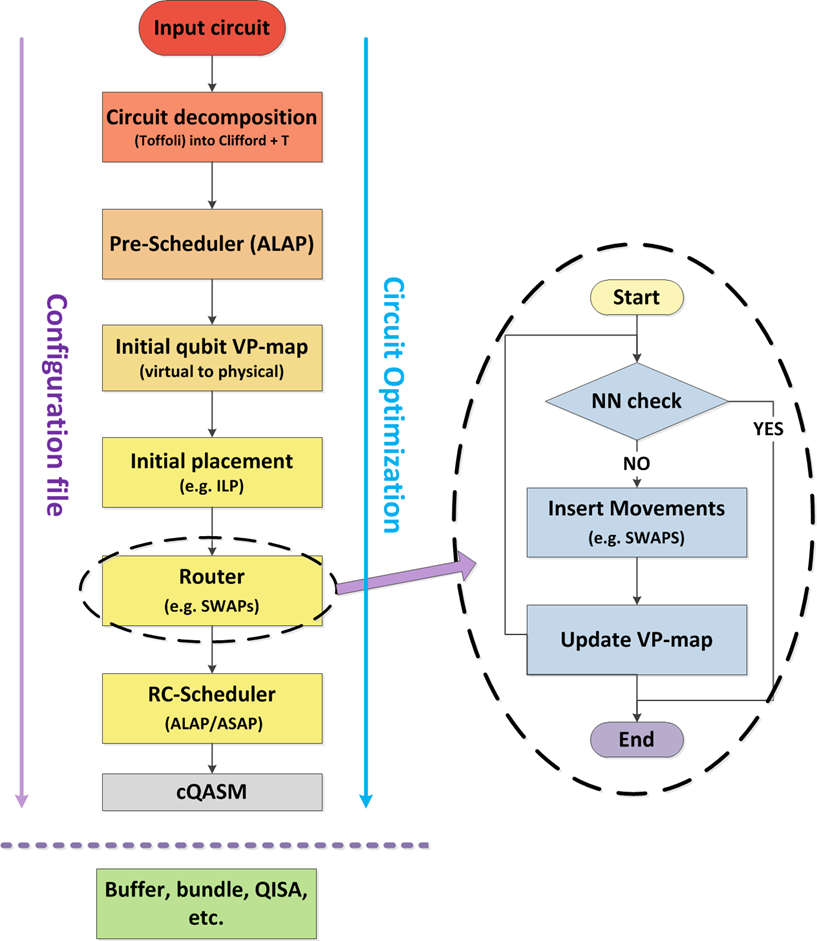
\includegraphics[width=0.5\textwidth]{figures/mapping_flow2.png}
\caption{\label{fig:orgafae7e3}
Mapping flow}
\end{figure}

\subsection*{Circuit decomposition}
\label{sec:org1587f46}

\subsection*{Pre-schedule}
\label{sec:org299d3a5}

\subsection*{Initial Virtual-to-Physical-map}
\label{sec:orgf0f914b}
\subsection*{Initial placement}
\label{sec:org8035d6e}
\subsection*{Router}
\label{sec:org6cfe608}
\subsection*{Resource constrains scheduler}
\label{sec:org89f971a}
One downside factor regarding this methodology is that the mapper only takes into account one cycle every time.
It does not look ahead in order to decide the best path also for next iterations.
Or, what is the same, it does not always find the best mapping solution.
This limitation comes from the fact that, the more steps you are looking ahead while mapping, the more computationally complex will be the mapper.
We highlight that the mapping problem is an NP problem with complexity \$O=\ldots{}\$.
Therefore, this method represents a viable solution, although a lot of future work should be done.

\section*{Mapping Metrics}
\label{sec:org76e0cb6}
As mentioned in the \href{chapter-2.org}{Mapping metrics} section in the second chapter, we name mapping metrics to those metrics used to assert the quality of a mapper.
In this section we will review the common metrics as the \textbf{number of SWAPs} or the \textbf{latency}, but we will also define -- and study in more detail -- some new mapping metrics that we incorporated, \textbf{probability of success} and \textbf{Quantum Volume}.

\subsection*{Number of SWAPs}
\label{sec:org7b206ed}

As explained before in the \href{chapter-2.org}{Mapping of quantum circuits} section, to route means to introduce SWAP operations -- or a decomposition of them.
Whenever a two-qubit gate requests two qubits that are far apart, a path in the gridlike chip layout should be given.
Each step on this grid would mean a SWAP operation between the vertex qubits of that step.
We already know that quantum gates are error prone and that one of the main problems that the mapping task is dealing with is to use the least amount of gates as possible.
Although the general mapping problem is to avoid the introduction of error to the original algorithm, that is caused by more sources apart from the number of gates.
Nonetheless, the quantum gates is one of the main error sources altogether with the decoherence time.
That is the reason why the number of SWAPs is commonly used to assert the quality of a mapper, but it is not enough.

\ldots{}

\subsection*{Latency}
\label{sec:org6bd2162}

Latency is the time required to run a quantum circuit in a given quantum device.
The introduction of gates due to the mapping makes the target circuit longer.
Or what is the same, the introduction of SWAPs -- or their decomposition -- adds several cycles to the depth of the circuit.
Therefore, the latency of the circuit increases.
For instance, \ldots{}

[Example from the mapping section with latency data]

One of the main source of errors is the decoherence, that is the quantum phenomena that makes the qubits loose their state along time.
The longer a quantum device is running an algorithm, the more errors would appear.
Or what is the same, the longer the circuit, the more erroneous will be the result.
The task of the scheduler -- one of the three mapping steps -- is to look for gates that can be run in parallel
Considering that time is one of the main error sources and that the scheduler task is to make operations simultaneously, one can understand why latency is used in order to assert the capacity of mapping algorithm
Nonetheless, as the number of SWAPs this metric is not giving enough information for that.

\ldots{}

\subsection*{Probability of success}
\label{sec:orgbd8c37f}

\begin{equation}
\label{eq:orga14353a}
{\displaystyle F(\rho ,\sigma )=\left(\operatorname {Tr} {\sqrt {{\sqrt {\rho }}\sigma {\sqrt {\rho }}}}\right)^{2},}
\end{equation}

where \(\rho =\sum _{i}p_{i}|i\rangle \langle i|\) and \(\sigma =\sum _{i}q_{i}|i\rangle \langle i|\).
These states are named \textbf{mixed states} and they are defined as the weighted sum of different pure states.
This is the general case in order to calculate the fidelity in any case.
But, for a situation with one of the states as pure state (\({\displaystyle \rho =|\psi _{\rho }\rangle \!\langle \psi _{\rho }|}\)) the calculation of fidelity reduces its complexity as it can be understood from eq. \ref{eq:org0fce9d5}.
Eq. \ref{eq:org700c0ed} the next step of simplicity, the one in which both states are pure (\({\displaystyle \rho =|\psi _{\rho }\rangle \!\langle \psi _{\rho }|}, {\displaystyle \sigma =|\psi _{\sigma }\rangle \!\langle \psi _{\sigma }|} {\displaystyle \sigma =|\psi _{\sigma }\rangle \!\langle \psi _{\sigma }|}\)).


\begin{equation}
\label{eq:org0fce9d5}
{\displaystyle F(\rho ,\sigma )=\operatorname {Tr} \left[{\sqrt {|\psi _{\rho }\rangle \langle \psi _{\rho }|\sigma |\psi _{\rho }\rangle \langle \psi _{\rho }|}}\right]^{2}=\langle \psi _{\rho }|\sigma |\psi _{\rho }\rangle \operatorname {Tr} \left[{\sqrt {|\psi _{\rho }\rangle \langle \psi _{\rho }|}}\right]^{2}=\langle \psi _{\rho }|\sigma |\psi _{\rho }\rangle .}
\end{equation}

\begin{equation}
\label{eq:org700c0ed}
{\displaystyle F(\rho ,\sigma )=|\langle \psi _{\rho }|\psi _{\sigma }\rangle |^{2}}
\end{equation}

\subsection*{Quantum Volume}
\label{sec:orgc3dc704}

Given the different hardware implementations and technologies in Quantum Computation (superconducting, ion-trap, spin qubits, \ldots{}), it is often difficult to benchmark the usefulness or power of quantum systems. 
A \textbf{hardware-independent measure} is required to depict whether a device is able to run a quantum circuit or not.
Here is where the Quantum Volume metric appears on the scene.

The aim of Quantum Volume is to quantify the computational power of quantum devices. 
Consequently we will use it as a metric to measure the runnability of the quantum algorithms and the quantum devices -- \emph{\textbf{"can this algorithm be run in a given device?"}}.
While the device is the basis of the Quantum Volume metric, we fix our attention on the circuit.
Our purpose is to assert how the mapping procedure affects the runnability of a given circuit and to study how the Quantum Volume is related to the probability of success.

\begin{itemize}
\item Definition
\label{sec:org929d0d3}

In this section, we define the Quantum Volume metric as well as the insights and ideas motivated by its capabilities

\begin{itemize}
\item Hardware parameters
\label{sec:org410e0f2}

The Quantum Volume metric considers that a quantum computer's performance mainly depends on the next hardware specifications:

\begin{itemize}
\item \(N\). The number of physical qubits
\item Quantum chip topology. The connectivity between qubits
\item Maximum number of sequential gates with correctable errors. The number of gates that can be applied before errors or decoherence mask the result
\item Gate set. Available hardware gate set
\item Maximum number of parallel operations. Number of operations that can be run in parallel
\end{itemize}

\item Definitions and metrics
\label{sec:org6d34f3d}

In order to understand the metric of Quantum Volume, some concepts need to be defined first. 
In this section we offer the inferred definitions from \cite{Bishop_2017,Moll_2018} that are part of the rationale of Quantum Volume.


\begin{description}
\item[{Model algorithm.}] In the literature, Bishop et al. use the term \emph{model algorithm} in \cite{Bishop_2017} to refer to a depth-one circuit, "constructed by random 2-qubit unitary matrix chosen uniformly over \(SU (4)\) on a random pairing of the qubits". Or, what is the same, the \emph{model algorithm} is a \emph{circuit unit} of depth one defined by a combination of any single- or two-qubit gates. The mapping requirements of the device and the mapping quality is included as well. In the case that a two-qubit gate force any qubit to be routed, the gate additions will be included in the \emph{model algorithm}. Therefore, we can say that it is device specific, as soon as it takes into account the constraints from it.
\end{description}

\begin{figure}[htbp]
\centering
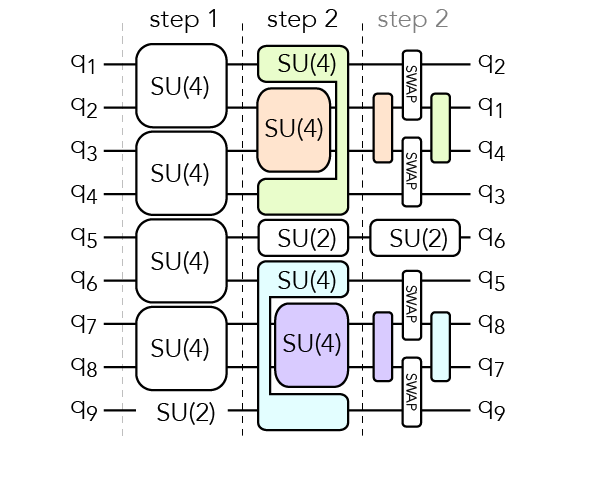
\includegraphics[width=0.7\textwidth]{figures/model_algorithm.png}
\caption{\label{fig:orga26090b}
Model algorithm example from \cite{Moll_2018}. Each step represents a possible combination of gates considered as \emph{model algorithm}. Notice that step 2 requires a mapping process that is shown afterwards.}
\end{figure}


\begin{description}
\item[{Active qubits (\(\textbf{n}\))}] Number of active qubits in a device of \(N\) qubits for a given algorithm.
\end{description}


\begin{description}
\item[{Effective error rate (\(\epsilon_{eff} \sim 1/(d(N) n)\)).}] It defines how well a device can implement arbitrary pairwise interactions between qubits. \(\epsilon_{eff}\) is the error rate per \emph{model algorithm}, an averaged error over many realizations of depth-one circuits conformed with random combinations of single- and two-qubit gates. It encapsulates errors of both single- and two-qubit gates. And it depends not only on the gate error rates, but also on the sophistication of the scheduling algorithm responsible of mapping the \emph{model algorithm} to the hardware.

\item[{Achievable circuit depth (\(d(N) \simeq \frac{1}{N \epsilon_{eff}}\))}] Maximum circuit depth for which the results, after running it on some device, are correctable and useful.
\end{description}

\begin{description}
\item[{(General) Quantum Volume (\(\tilde{V}_Q = min (N, d(N))^2\))}] quantifies the space-time volume occupied by a \emph{model algorithm} with random two-qubit gates that can be reliably executed on a given device.
\end{description}

\item Runnability
\label{sec:org12bdf52}

After understading the concept of Quantum Volume, we derived some insights and we had ideas motivated by the possibilities that this new metric offers. 
We define the \textbf{runnability} of a given quantum circuit on a device based on the separation of the concepts of \emph{device} Quantum Volume (\(V_Q\)) and \emph{algorithm} Quantum Volume (\(V^a_Q\)).


\begin{itemize}
\item Quantum Volume of a device
\label{sec:org3dd08f5}

Following \cite{Bishop_2017,Moll_2018}, we can expand the Quantum Volume general equation (\(\tilde{V}_Q\)) with the other definitions in the previous section and maximize for the biggest possible \(n\) in the device. 
Then, the maximum Quantum Volume that a device could run is defined by:

\begin{equation}
\label{eq:org6197d63}
V_Q = \max_{n \le N} \min \left[ n,\frac{1}{n \epsilon_{eff} (n)}\right]^2
\end{equation}

We define this as the \emph{device} Quantum Volume. 
In Fig. \ref{fig:deviceQV} a graph describing the Quantum Volume as a function of \(n\) and \(\epsilon_{eff}\) is shown.
For this example we are not considering \(\epsilon_{eff} (n)\).
Otherwise, it would be a technology specific graph.
The purpose of this figure is tho show the general behaviour of \(V_Q\).
Note that the axis are in a logarithmic scale in order to show that \(V_Q\) grows exponentially as \(n\) increase and that \(\epsilon_{eff}\) is abruptly detonating \(V_Q\) growth from values smaller than \(10^{-3}\).
Therefore, we outline that the main limit for the \(V_Q\) is the \(\epsilon_{eff}\).

\begin{figure}[htbp]
\centering
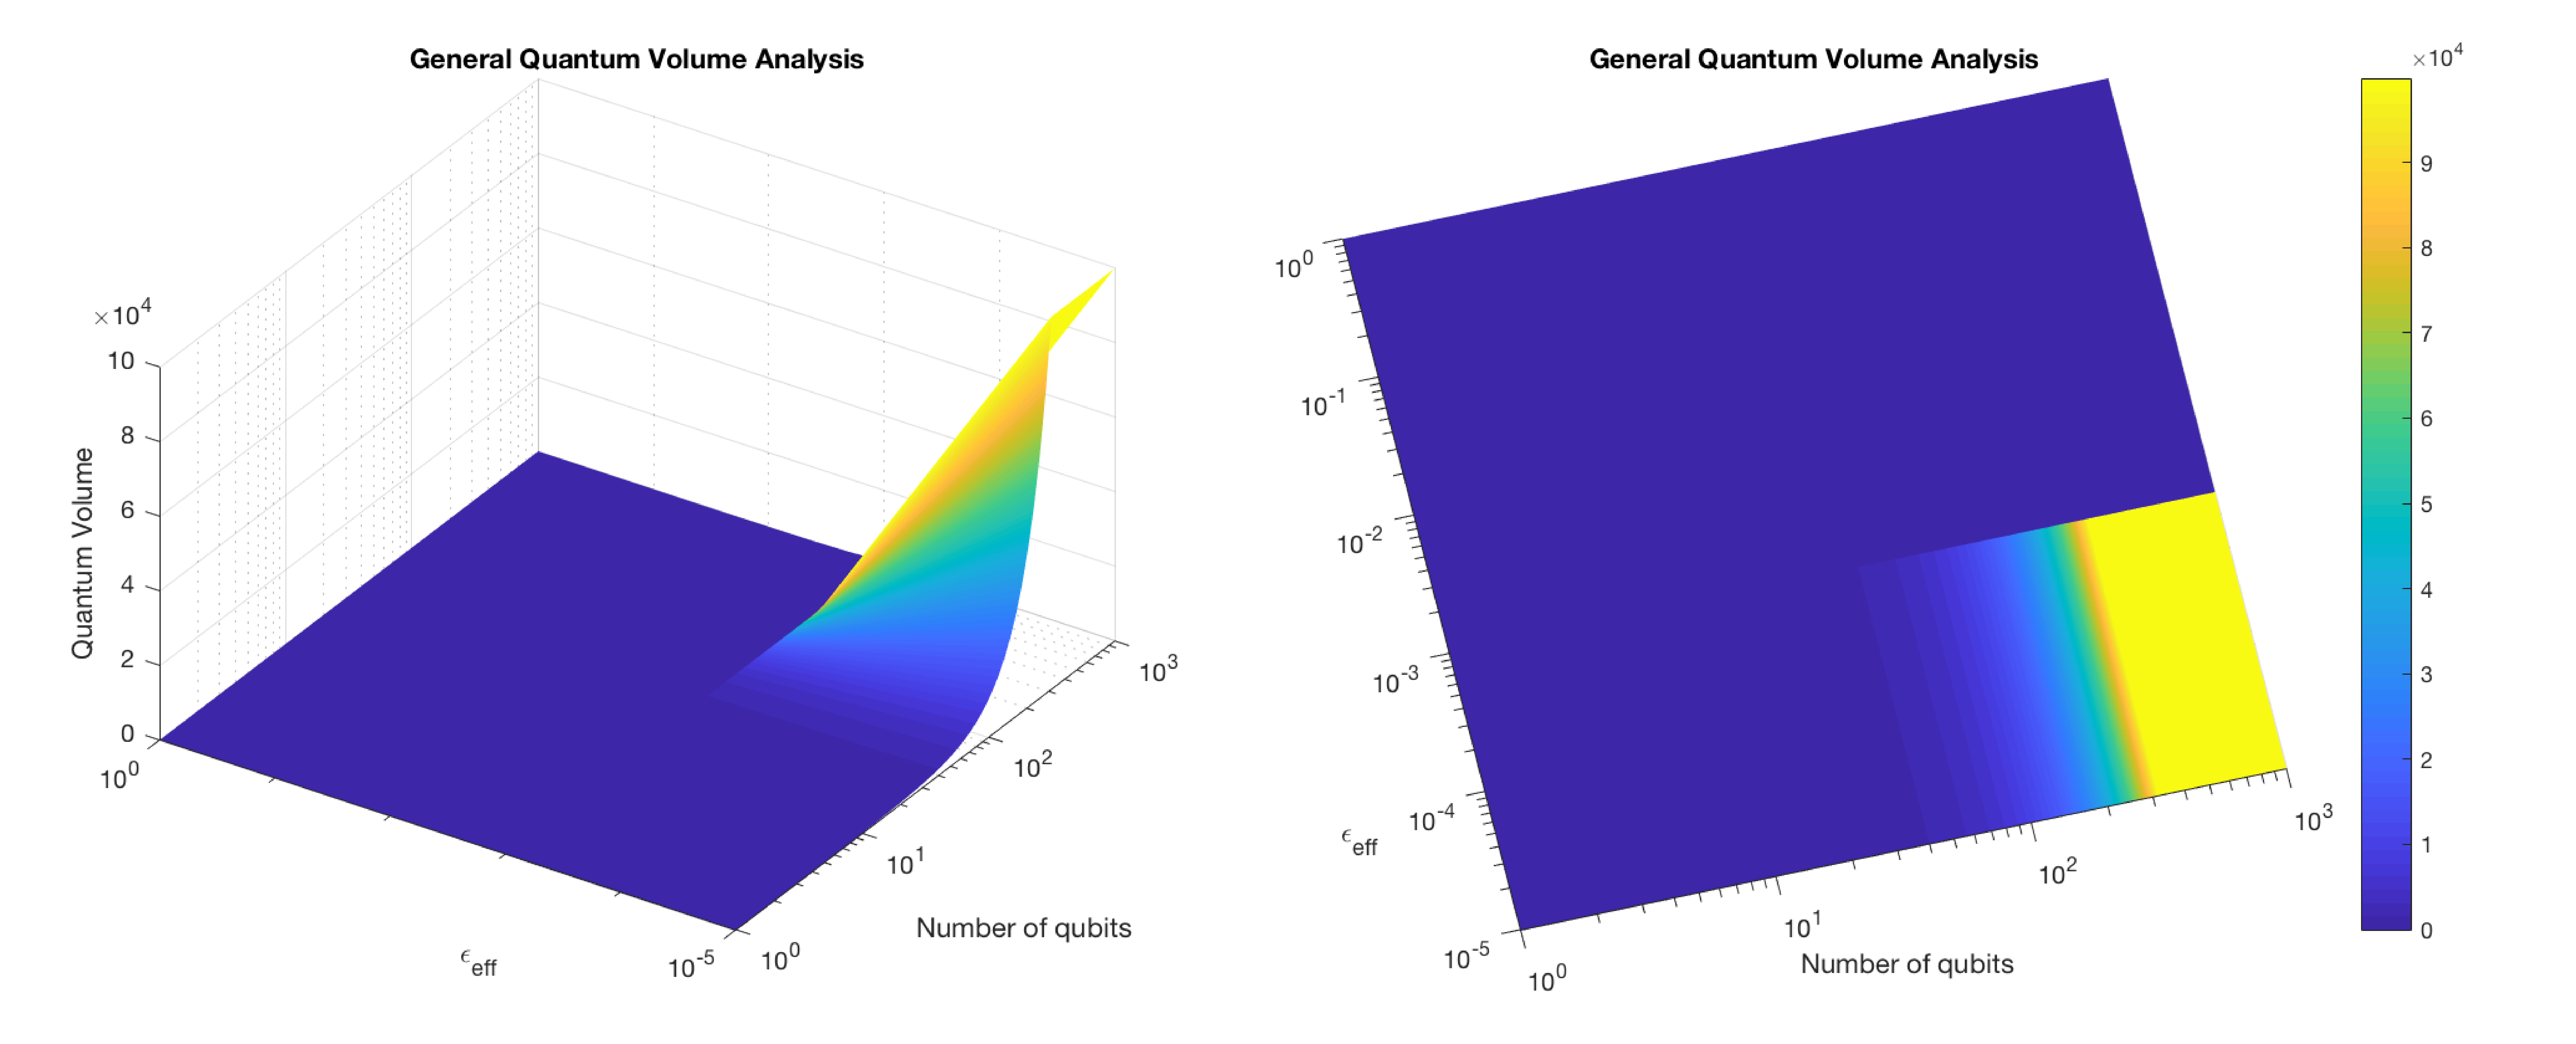
\includegraphics[width=\textwidth]{figures/general_QV.png}
\caption{\label{fig:orgf252150}
Device Quantum Volume behaviour for values less than 1000 qubits and a \(\epsilon_eff < 10^{-5}\)}
\end{figure}

\item Quantum Volume of an algorithm
\label{sec:org677a1e3}

As with \(V_Q\), we initially defined the algorithm's Quantum Volume from the general equation \(\tilde{V}_Q\), although we will adapt it later.

\begin{equation}
\label{eq:orgadbebdb}
V_Q^a = \min \left[ n,d \right]^2
\end{equation}

Note that \(d\) is not \(d(N)\) but the real depth of the given algorithm.
At the same time, \(n\) is the number of qubits required by the algorithm itself.
One can see how \(d\) and \(n\) are equally important in Fig. \ref{fig:algorithmQVsym}.
The growth of both variables causes an equally exponential growth of \(V^a_Q\).

\begin{figure}[htbp]
\centering
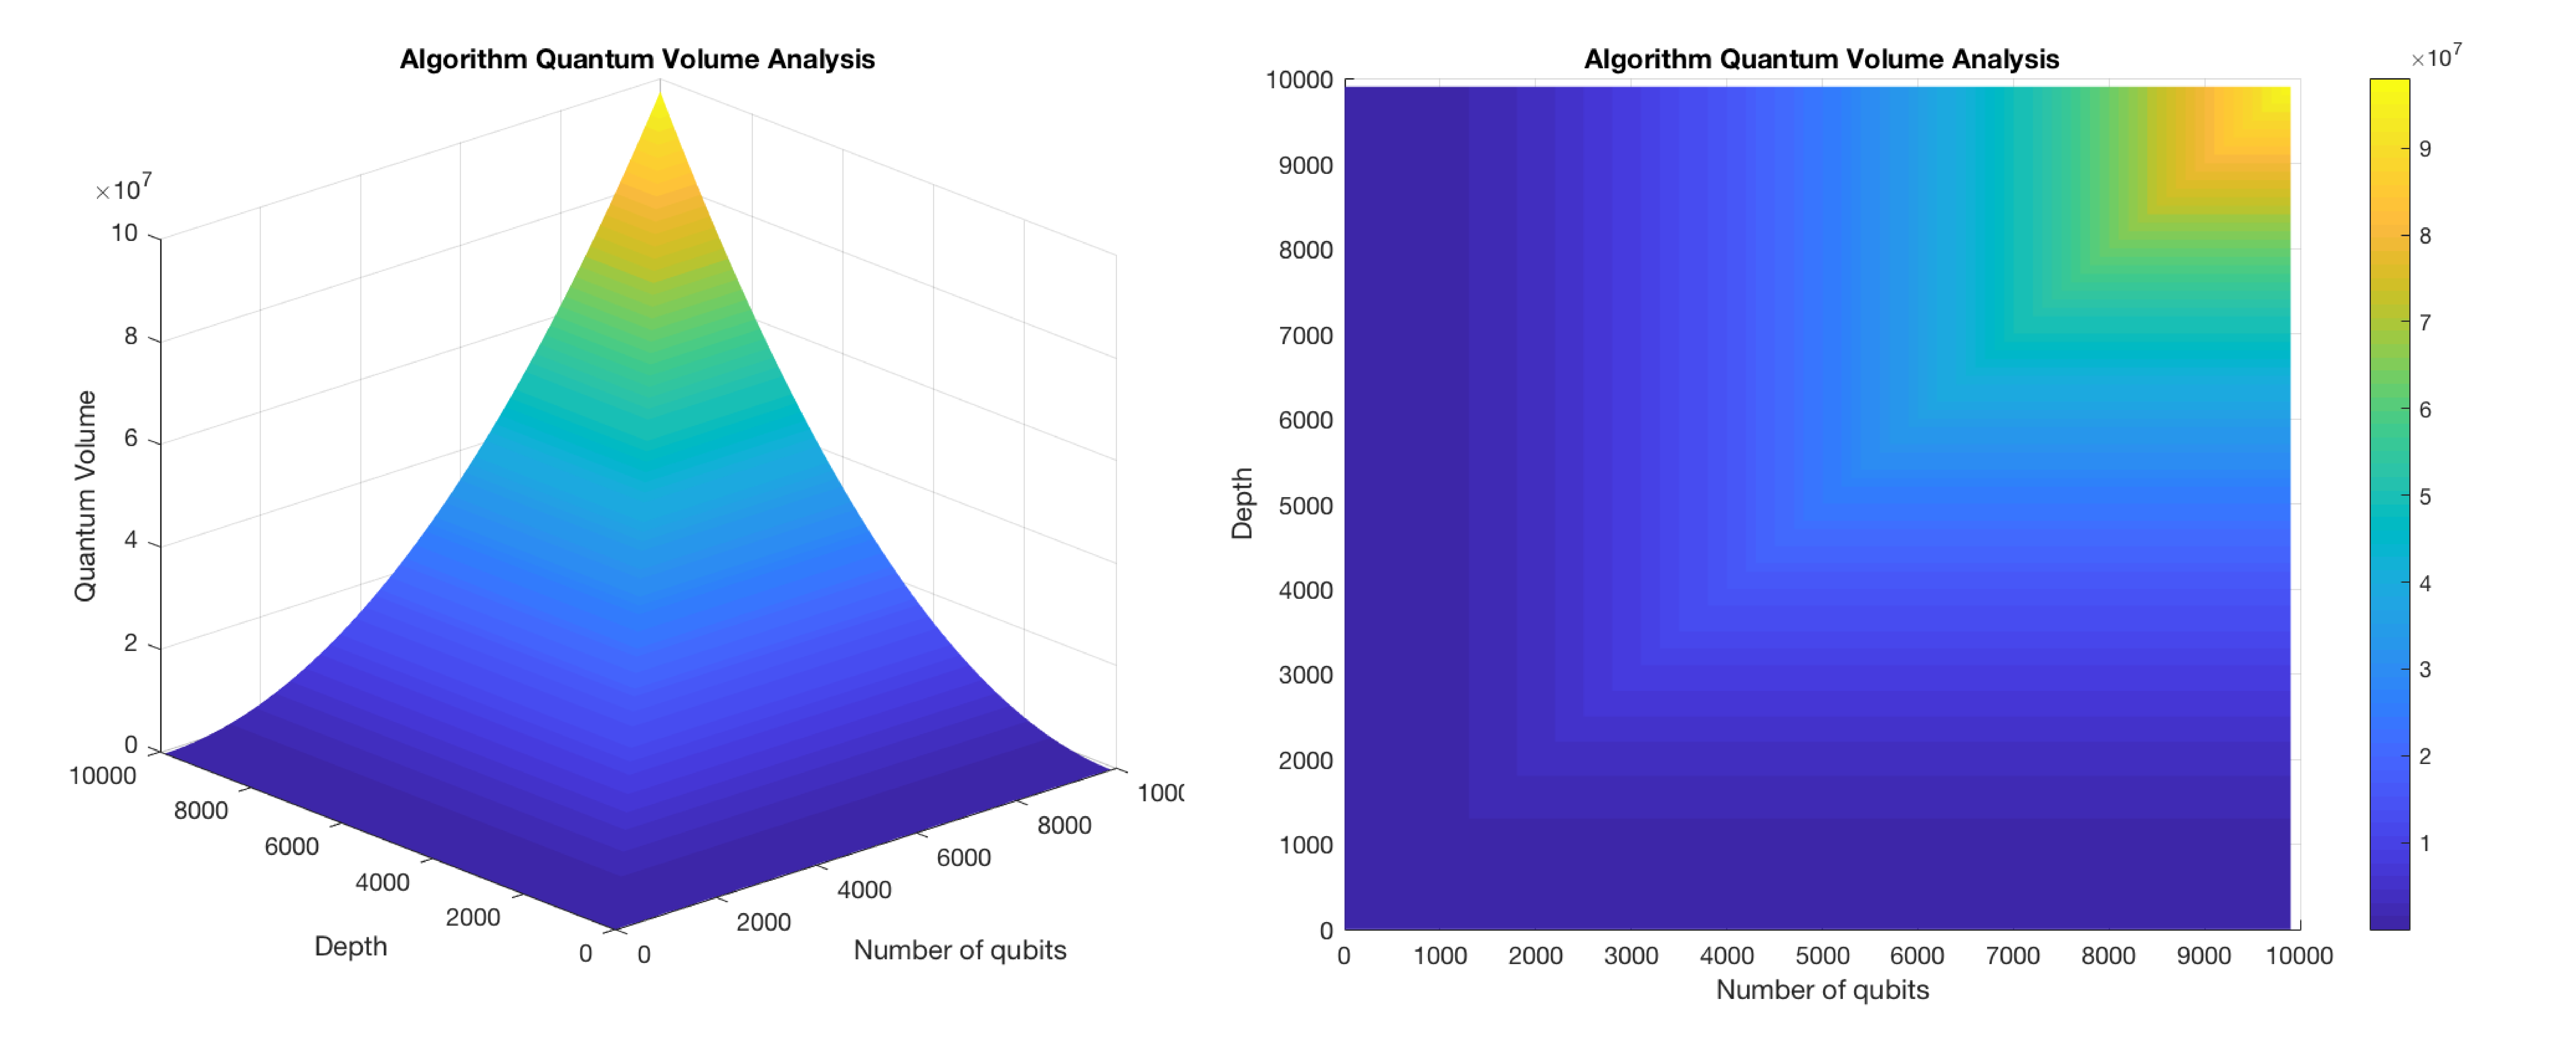
\includegraphics[width=\textwidth]{figures/V_q_analysis_sym.png}
\caption{\label{fig:orgb76dd98}
Algorithm Quantum Volume as in eq. \ref{eq:orgadbebdb} behaviour for values less than \(10^{4}\) qubits and depth less than \(10^{4}\)}
\end{figure}

Fig. \ref{fig:algorithmQVasym} present the behaviour of \(V_Q^a\)
focusing in the current most common values for \(n\) and \(d\).
The function shows an asymteric beheviour due to \(d\) is much bigger than \(n\) most of the times.


\begin{figure}[htbp]
\centering
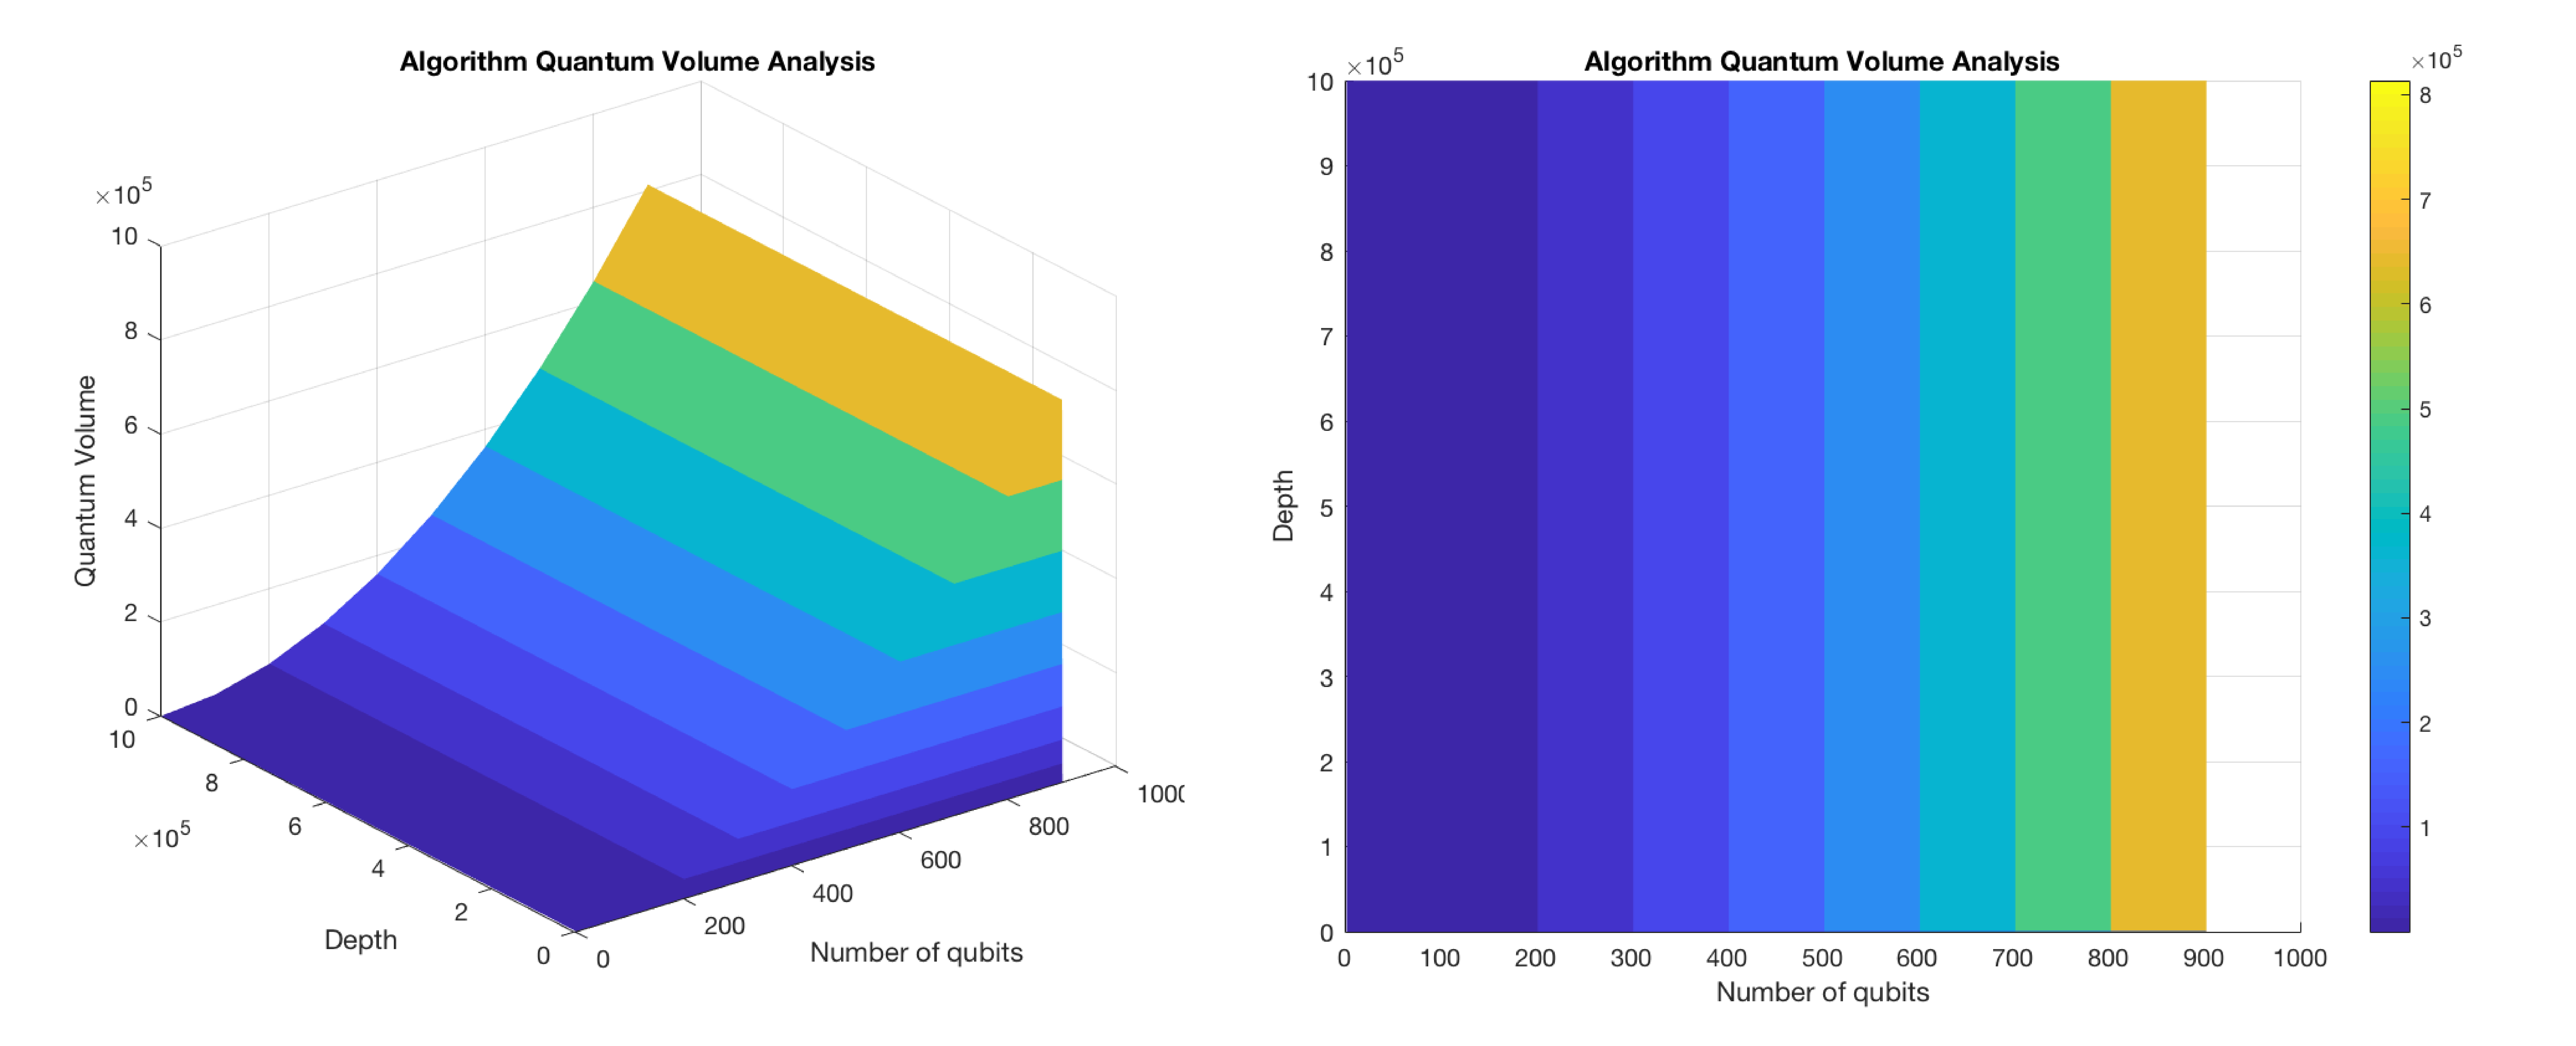
\includegraphics[width=\textwidth]{figures/V_q_analysis_asym.png}
\caption{\label{fig:orgb01087f}
Algorithm Quantum Volume as in eq. \ref{eq:orgadbebdb} behaviour for values less than 1000 qubits and a depth less than \(10^{5}\)}
\end{figure}

We aware that this approach has a limitation regarding the mapping of the quantum circuit.
As explained before, \(V_Q\) is able to take into account the sophistication of the mapping procedure.
It is inherited in the \emph{model algorithm}.
But, in this case, the \(V^a_Q\) of an algorithm before and after mapping will remain the same.
After mapping an algorithm, the usual effect is an increase in the depth or the number of operations.
Rare mapping methods consider the qubit addition in the technique.
And, even considering it, \(n\) is not often growing too much in comparison with \(d\).
In the current NISQ era, the quantum circuits need much less qubits than depth.
Therefore, most of the times, the minimum value between \(n\) and \(d\) will be \(n\).
As soon as \(V^a_Q\) is taking into account the minimum of them and the mapping procedure affects mostly to \(d\) we can conclude that this definition of \(V^a_Q\) is not considering the mapping in its results.

A simplified solution for this problem would be the \(V^a_Q\) definition as the multiplication between \(n\) and \(d\).
Unfortunately, this approach has several drawbacks as well.
As Moll et al. point out \cite{Moll_2018}, extreme cases of high \(n\) and low \(d\) -- or the other way around -- lead to inconsistencies of the multiplication metric.
But, considering that most of our work is not going to be in any of these extreme cases and that we can avoid those outliers, we define the algorithm's Quantum Volume as:

\begin{equation}
\label{eq:orge1bb3e1}
V_Q^a =  n \times d
\end{equation}

Fig. \ref{fig:algorithmmultQV} report the behaviour of the \(V_Q^a\) as
the multiplication of \(n\) and \(d\).
As illutrated in Fig. \ref{fig:algorithmQVsym}, the values of \(n\) and \(d\) are
affecting equally and exponentially to the metric.

\begin{figure}[htbp]
\centering
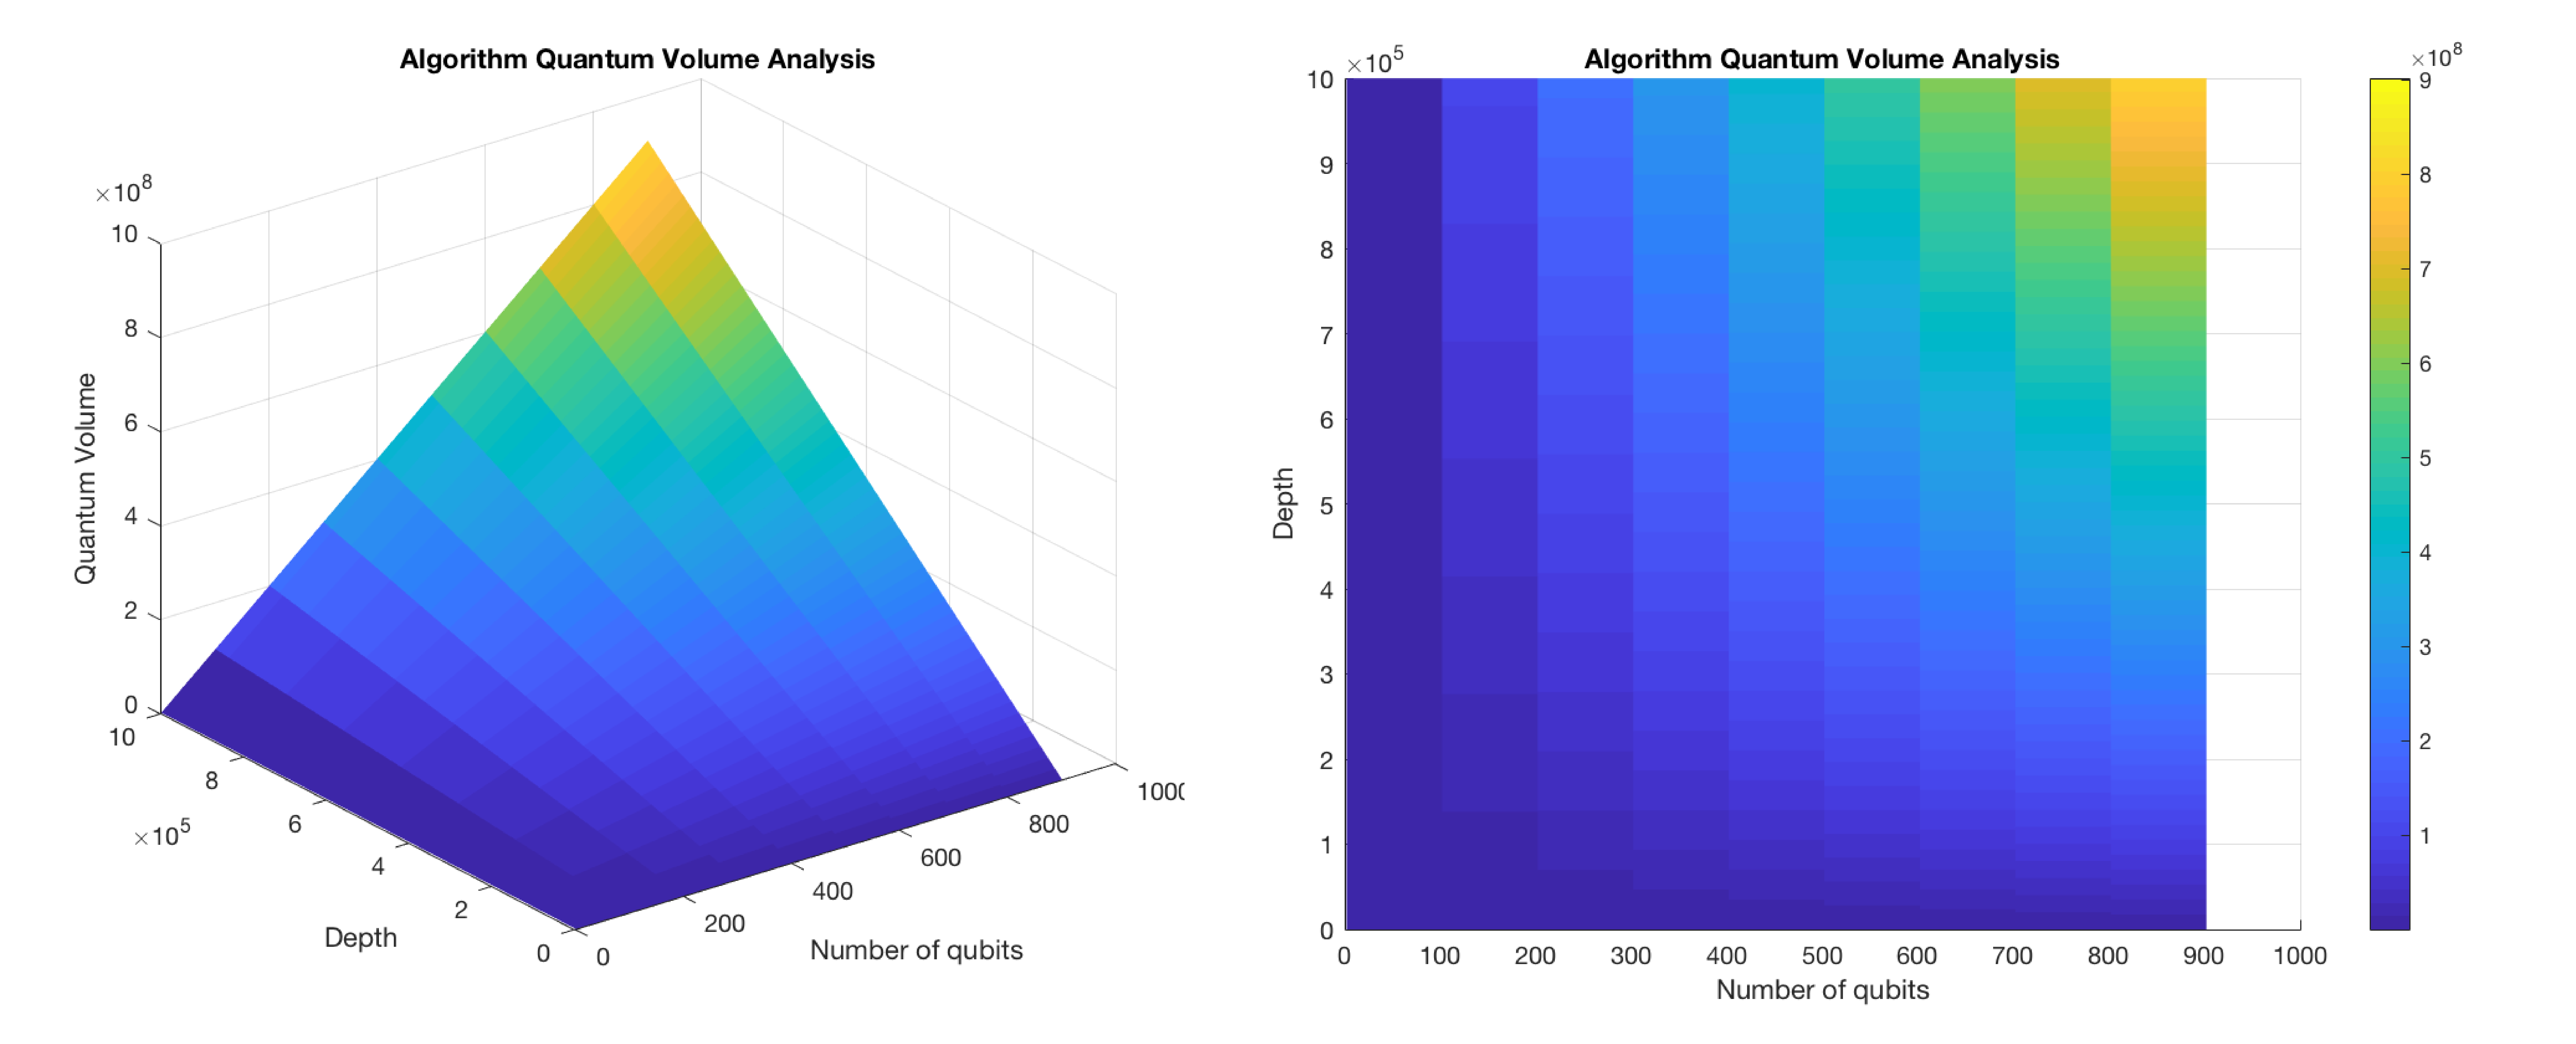
\includegraphics[width=\textwidth]{figures/V_q_analysis_mult.png}
\caption{\label{fig:org9651c87}
Algorithm Quantum Volume as in eq. \ref{eq:orge1bb3e1} behaviour for values less than 1000 qubits and a depth less than \(10^{5}\)}
\end{figure}

\item Runnability
\label{sec:orgf6245ef}

Finally, once the Quantum Volume of device and algorithm are stated, we define runnability as the condition for which the \(V_Q\) should be bigger than \(V^a_Q\).
That is the condition that the computational power of the device should be bigger than the computational power required by the algorithm.

$$\text{Runnable if: } V_Q > V^a_Q \quad \quad \text{ when } N \ge n$$

For instance, in order to understand this concept, one may imagine the process of checking, whether or not, some cube with a given volume -- representing the algorithm -- would fit in a box -- the device --.
If the algorithm's box volume is smaller than the volume of the device's box, the algorithm's box will fit inside.

Indeed, one acceptable criticism of this definition is that, as \(V_Q\) and \(V^a_Q\) are finally defined in the previous sections, it seems that it is not really fair to compare them.
But, as soon as the general behaviour of the final and the initial \(V^a_Q\) is the same -- one can see in the Fig. \ref{fig:algorithmQVsym} and Fig. \ref{fig:algorithmmultQV} -- and as the final definition tends to have bigger values than the initial one -- so it is defining a more restrictive and exigent scenario -- we believe that this definition of runnability is mathematically correct and useful.

Therefore, we define runnability as the condition of:

\begin{equation}
\label{eq:org5441b51}
\max_{n \le N} \min \left[ n,\frac{1}{n \epsilon_{eff} (n)}\right]^2 > n \times d \quad \quad \text{ when } N \ge n
\end{equation}
\end{itemize}
\end{itemize}

\item Methodology
\label{sec:org0522931}

After explaining the insights and our new concepts around the metric of Quantum Volume, let us now
look at our methodology.
One issue that needs to be raised is the difficulty of the \(\epsilon_{eff}\) calculation for a device.
In our work, we will try to avoid this exhausting process outlining how much computational power
is required by a given algorithm.
Or, in other words, we will calculate the \(V^a_Q\) and assert that it would be able to run in devices
with \(V_Q > V^a_Q\).
\(V^a_Q\) will be a threshold to define the runnability of a given algorithm.

As mentioned at the beginning, we are also interested on the impact of the mapping step in the
Quantum Volume.
Because of that, we will check the differences of \(V^a_Q\) in the same circuit, before and after
mapping it.
We are concerned about the relation between Quantum Volume and the probability of success, as
well.
We will analyze the results of both metrics, thus.

Subsequently, the design of our Quantum Volume method will follow the next stages.
First, given a quantum algorithm, we will calculate the Quantum Volume of a circuit, before and after mapping.
Then, we will compare both results and we will investigate their relationship with the probability
of success, if any.
Finally, we will outline the runnability threshold of the algorithm.

\begin{table}[htbp]
\caption{\label{tab:org87bc1cf}
Summary of the steps to outline the range of possible values for running a given algorithm}
\centering
\small
\begin{tabular}{|l|}
\hline
\\
Steps:\\
\\
1. Calculation of \(V^a_Q \prime\) for a given algorithm without mapping\\
2. Calculation of \(V^a_Q\) for a given algorithm after being mapped with the constraints of some device\\
3. Compare \(V^a_Q \prime\) and \(V^a_Q\)\\
4. Look for relation with probability of success\\
5. Threshold \(V_Q\) with \(V^a_Q\) (\(V_Q > V^a_Q\) and \(N \ge n\))\\
\\
\hline
\end{tabular}
\end{table}
\end{itemize}
